% Options for packages loaded elsewhere
\PassOptionsToPackage{unicode}{hyperref}
\PassOptionsToPackage{hyphens}{url}
%
\documentclass[
]{article}
\usepackage{amsmath,amssymb}
\usepackage{lmodern}
\usepackage{iftex}
\ifPDFTeX
  \usepackage[T1]{fontenc}
  \usepackage[utf8]{inputenc}
  \usepackage{textcomp} % provide euro and other symbols
\else % if luatex or xetex
  \usepackage{unicode-math}
  \defaultfontfeatures{Scale=MatchLowercase}
  \defaultfontfeatures[\rmfamily]{Ligatures=TeX,Scale=1}
\fi
% Use upquote if available, for straight quotes in verbatim environments
\IfFileExists{upquote.sty}{\usepackage{upquote}}{}
\IfFileExists{microtype.sty}{% use microtype if available
  \usepackage[]{microtype}
  \UseMicrotypeSet[protrusion]{basicmath} % disable protrusion for tt fonts
}{}
\makeatletter
\@ifundefined{KOMAClassName}{% if non-KOMA class
  \IfFileExists{parskip.sty}{%
    \usepackage{parskip}
  }{% else
    \setlength{\parindent}{0pt}
    \setlength{\parskip}{6pt plus 2pt minus 1pt}}
}{% if KOMA class
  \KOMAoptions{parskip=half}}
\makeatother
\usepackage{xcolor}
\usepackage[margin=1in]{geometry}
\usepackage{color}
\usepackage{fancyvrb}
\newcommand{\VerbBar}{|}
\newcommand{\VERB}{\Verb[commandchars=\\\{\}]}
\DefineVerbatimEnvironment{Highlighting}{Verbatim}{commandchars=\\\{\}}
% Add ',fontsize=\small' for more characters per line
\usepackage{framed}
\definecolor{shadecolor}{RGB}{248,248,248}
\newenvironment{Shaded}{\begin{snugshade}}{\end{snugshade}}
\newcommand{\AlertTok}[1]{\textcolor[rgb]{0.94,0.16,0.16}{#1}}
\newcommand{\AnnotationTok}[1]{\textcolor[rgb]{0.56,0.35,0.01}{\textbf{\textit{#1}}}}
\newcommand{\AttributeTok}[1]{\textcolor[rgb]{0.77,0.63,0.00}{#1}}
\newcommand{\BaseNTok}[1]{\textcolor[rgb]{0.00,0.00,0.81}{#1}}
\newcommand{\BuiltInTok}[1]{#1}
\newcommand{\CharTok}[1]{\textcolor[rgb]{0.31,0.60,0.02}{#1}}
\newcommand{\CommentTok}[1]{\textcolor[rgb]{0.56,0.35,0.01}{\textit{#1}}}
\newcommand{\CommentVarTok}[1]{\textcolor[rgb]{0.56,0.35,0.01}{\textbf{\textit{#1}}}}
\newcommand{\ConstantTok}[1]{\textcolor[rgb]{0.00,0.00,0.00}{#1}}
\newcommand{\ControlFlowTok}[1]{\textcolor[rgb]{0.13,0.29,0.53}{\textbf{#1}}}
\newcommand{\DataTypeTok}[1]{\textcolor[rgb]{0.13,0.29,0.53}{#1}}
\newcommand{\DecValTok}[1]{\textcolor[rgb]{0.00,0.00,0.81}{#1}}
\newcommand{\DocumentationTok}[1]{\textcolor[rgb]{0.56,0.35,0.01}{\textbf{\textit{#1}}}}
\newcommand{\ErrorTok}[1]{\textcolor[rgb]{0.64,0.00,0.00}{\textbf{#1}}}
\newcommand{\ExtensionTok}[1]{#1}
\newcommand{\FloatTok}[1]{\textcolor[rgb]{0.00,0.00,0.81}{#1}}
\newcommand{\FunctionTok}[1]{\textcolor[rgb]{0.00,0.00,0.00}{#1}}
\newcommand{\ImportTok}[1]{#1}
\newcommand{\InformationTok}[1]{\textcolor[rgb]{0.56,0.35,0.01}{\textbf{\textit{#1}}}}
\newcommand{\KeywordTok}[1]{\textcolor[rgb]{0.13,0.29,0.53}{\textbf{#1}}}
\newcommand{\NormalTok}[1]{#1}
\newcommand{\OperatorTok}[1]{\textcolor[rgb]{0.81,0.36,0.00}{\textbf{#1}}}
\newcommand{\OtherTok}[1]{\textcolor[rgb]{0.56,0.35,0.01}{#1}}
\newcommand{\PreprocessorTok}[1]{\textcolor[rgb]{0.56,0.35,0.01}{\textit{#1}}}
\newcommand{\RegionMarkerTok}[1]{#1}
\newcommand{\SpecialCharTok}[1]{\textcolor[rgb]{0.00,0.00,0.00}{#1}}
\newcommand{\SpecialStringTok}[1]{\textcolor[rgb]{0.31,0.60,0.02}{#1}}
\newcommand{\StringTok}[1]{\textcolor[rgb]{0.31,0.60,0.02}{#1}}
\newcommand{\VariableTok}[1]{\textcolor[rgb]{0.00,0.00,0.00}{#1}}
\newcommand{\VerbatimStringTok}[1]{\textcolor[rgb]{0.31,0.60,0.02}{#1}}
\newcommand{\WarningTok}[1]{\textcolor[rgb]{0.56,0.35,0.01}{\textbf{\textit{#1}}}}
\usepackage{graphicx}
\makeatletter
\def\maxwidth{\ifdim\Gin@nat@width>\linewidth\linewidth\else\Gin@nat@width\fi}
\def\maxheight{\ifdim\Gin@nat@height>\textheight\textheight\else\Gin@nat@height\fi}
\makeatother
% Scale images if necessary, so that they will not overflow the page
% margins by default, and it is still possible to overwrite the defaults
% using explicit options in \includegraphics[width, height, ...]{}
\setkeys{Gin}{width=\maxwidth,height=\maxheight,keepaspectratio}
% Set default figure placement to htbp
\makeatletter
\def\fps@figure{htbp}
\makeatother
\setlength{\emergencystretch}{3em} % prevent overfull lines
\providecommand{\tightlist}{%
  \setlength{\itemsep}{0pt}\setlength{\parskip}{0pt}}
\setcounter{secnumdepth}{-\maxdimen} % remove section numbering
\ifLuaTeX
  \usepackage{selnolig}  % disable illegal ligatures
\fi
\IfFileExists{bookmark.sty}{\usepackage{bookmark}}{\usepackage{hyperref}}
\IfFileExists{xurl.sty}{\usepackage{xurl}}{} % add URL line breaks if available
\urlstyle{same} % disable monospaced font for URLs
\hypersetup{
  pdftitle={Homework 2},
  pdfauthor={Ryan Wang},
  hidelinks,
  pdfcreator={LaTeX via pandoc}}

\title{Homework 2}
\author{Ryan Wang}
\date{}

\begin{document}
\maketitle

{
\setcounter{tocdepth}{2}
\tableofcontents
}
\hypertarget{linear-regression-and-knn}{%
\subsection{Linear Regression and KNN}\label{linear-regression-and-knn}}

For this assignment, we will be working with a data set from the UCI
(University of California, Irvine) Machine Learning repository
(\href{http://archive.ics.uci.edu/ml/datasets/Abalone}{see website
here}). The full data set consists of \(4,177\) observations of abalone
in Tasmania. (Fun fact:
\href{https://en.wikipedia.org/wiki/Tasmania}{Tasmania} supplies about
\(25\%\) of the yearly world abalone harvest.)

\begin{figure}
\centering
\includegraphics[width=1.58333in,height=\textheight]{https://cdn.shopify.com/s/files/1/1198/8002/products/1d89434927bffb6fd1786c19c2d921fb_2000x_652a2391-5a0a-4f10-966c-f759dc08635c_1024x1024.jpg?v=1582320404}
\caption{\emph{Fig 1. Inside of an abalone shell.}}
\end{figure}

The age of an abalone is typically determined by cutting the shell open
and counting the number of rings with a microscope. The purpose of this
data set is to determine whether abalone age (\textbf{number of rings +
1.5}) can be accurately predicted using other, easier-to-obtain
information about the abalone.

The full abalone data set is located in the
\texttt{\textbackslash{}data} subdirectory. Read it into \emph{R} using
\texttt{read\_csv()}. Take a moment to read through the codebook
(\texttt{abalone\_codebook.txt}) and familiarize yourself with the
variable definitions.

Make sure you load the \texttt{tidyverse} and \texttt{tidymodels}!

\hypertarget{question-1}{%
\subsubsection{Question 1}\label{question-1}}

Your goal is to predict abalone age, which is calculated as the number
of rings plus 1.5. Notice there currently is no \texttt{age} variable in
the data set. Add \texttt{age} to the data set.

Assess and describe the distribution of \texttt{age}.

\begin{Shaded}
\begin{Highlighting}[]
\NormalTok{abalone }\OtherTok{\textless{}{-}} \FunctionTok{read.csv}\NormalTok{(}\FunctionTok{here}\NormalTok{(}\StringTok{\textquotesingle{}data\textquotesingle{}}\NormalTok{, }\StringTok{"abalone.csv"}\NormalTok{))}
\NormalTok{abalone }\OtherTok{\textless{}{-}} \FunctionTok{mutate}\NormalTok{(abalone, }\AttributeTok{age =}\NormalTok{ rings }\SpecialCharTok{+} \FloatTok{1.5}\NormalTok{) }\CommentTok{\# add age = ring + 1.5 to the data set.}


\FunctionTok{ggplot}\NormalTok{(}\AttributeTok{data =}\NormalTok{ abalone, }\FunctionTok{aes}\NormalTok{(age))}\SpecialCharTok{+}\FunctionTok{geom\_histogram}\NormalTok{(}\AttributeTok{bins=}\DecValTok{30}\NormalTok{)}
\end{Highlighting}
\end{Shaded}

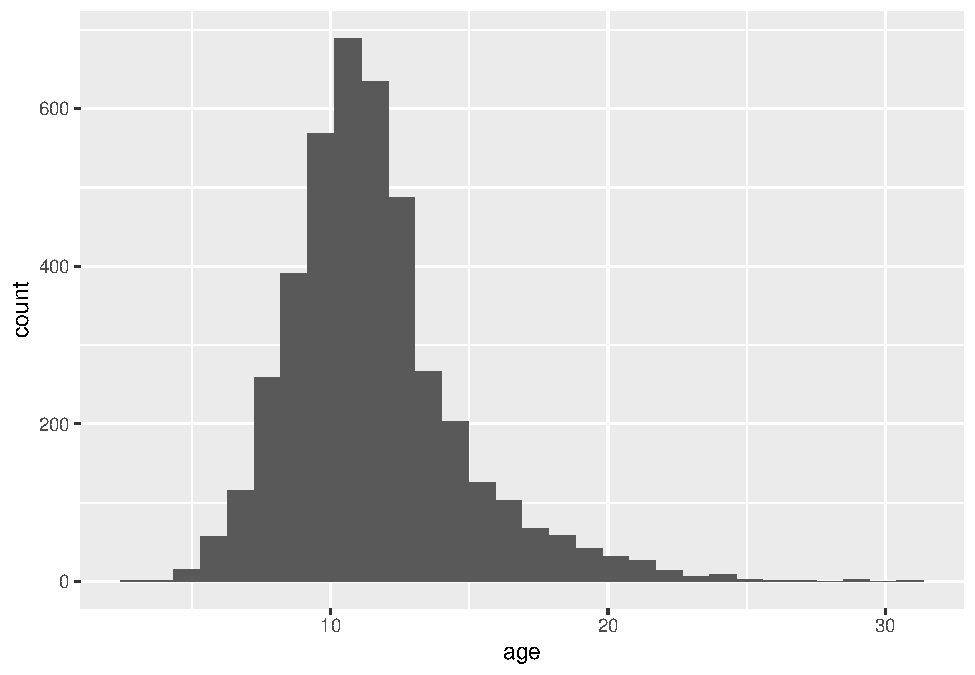
\includegraphics{homework-2_files/figure-latex/unnamed-chunk-1-1.pdf}

The plot shows that the distribution of age is approximately normal with
mean of 12 but it also some what skew to the right. The most of the data
locates between age of 4 and 16 and there exist outliers that have age
around 30.

\hypertarget{question-2}{%
\subsubsection{Question 2}\label{question-2}}

Split the abalone data into a training set and a testing set. Use
stratified sampling. You should decide on appropriate percentages for
splitting the data.

\emph{Remember that you'll need to set a seed at the beginning of the
document to reproduce your results.}

\begin{Shaded}
\begin{Highlighting}[]
\FunctionTok{set.seed}\NormalTok{(}\DecValTok{131}\NormalTok{)}
\NormalTok{abalone\_split }\OtherTok{\textless{}{-}} \FunctionTok{initial\_split}\NormalTok{(abalone,}\AttributeTok{prop=}\FloatTok{0.80}\NormalTok{,}\AttributeTok{strata =}\NormalTok{ age)}
\NormalTok{abalone\_train }\OtherTok{\textless{}{-}} \FunctionTok{training}\NormalTok{(abalone\_split)}
\NormalTok{abalone\_test }\OtherTok{\textless{}{-}} \FunctionTok{testing}\NormalTok{(abalone\_split)}
\end{Highlighting}
\end{Shaded}

\hypertarget{question-3}{%
\subsubsection{Question 3}\label{question-3}}

Using the \textbf{training} data, create a recipe predicting the outcome
variable, \texttt{age}, with all other predictor variables. Note that
you \textbf{should not} include \texttt{rings} to predict \texttt{age}.
\emph{Explain why you shouldn't use \texttt{rings} to predict
\texttt{age}.}

Steps for your recipe:

\begin{enumerate}
\def\labelenumi{\arabic{enumi}.}
\item
  dummy code any categorical predictors
\item
  create interactions between

  \begin{itemize}
  \tightlist
  \item
    \texttt{type} and \texttt{shucked\_weight},
  \item
    \texttt{longest\_shell} and \texttt{diameter},
  \item
    \texttt{shucked\_weight} and \texttt{shell\_weight}
  \end{itemize}
\item
  center all predictors, and
\item
  scale all predictors.
\end{enumerate}

You'll need to investigate the \texttt{tidymodels} documentation to find
the appropriate step functions to use.

\begin{Shaded}
\begin{Highlighting}[]
\NormalTok{abalone\_train\_no\_rings }\OtherTok{\textless{}{-}}\NormalTok{ abalone\_train}\SpecialCharTok{\%\textgreater{}\%} \FunctionTok{select}\NormalTok{(}\SpecialCharTok{{-}}\NormalTok{rings) }\CommentTok{\# exclude rings}

\NormalTok{abalone\_recipe }\OtherTok{\textless{}{-}} \FunctionTok{recipe}\NormalTok{(age }\SpecialCharTok{\textasciitilde{}}\NormalTok{ ., }\AttributeTok{data =}\NormalTok{ abalone\_train\_no\_rings) }\SpecialCharTok{\%\textgreater{}\%} 
  \FunctionTok{step\_dummy}\NormalTok{(}\FunctionTok{all\_nominal\_predictors}\NormalTok{()) }\SpecialCharTok{\%\textgreater{}\%}   \CommentTok{\# dummy code the categorical predictors}
  \FunctionTok{step\_interact}\NormalTok{(}\AttributeTok{terms =} \SpecialCharTok{\textasciitilde{}} \FunctionTok{starts\_with}\NormalTok{(}\StringTok{"type"}\NormalTok{)}\SpecialCharTok{:}\NormalTok{shucked\_weight }\SpecialCharTok{+}  \CommentTok{\# dummy variables }
\NormalTok{                  longest\_shell}\SpecialCharTok{:}\NormalTok{diameter }\SpecialCharTok{+}   
\NormalTok{                 shucked\_weight}\SpecialCharTok{:}\NormalTok{shell\_weight) }\SpecialCharTok{\%\textgreater{}\%}  \CommentTok{\# create interactions}
  
  \FunctionTok{step\_center}\NormalTok{(}\FunctionTok{all\_predictors}\NormalTok{()) }\SpecialCharTok{\%\textgreater{}\%}  \CommentTok{\# center predictors}
  
  \FunctionTok{step\_scale}\NormalTok{(}\FunctionTok{all\_predictors}\NormalTok{())  }\CommentTok{\# scale predictors}
\end{Highlighting}
\end{Shaded}

We should not include `rings' in predicting `age' because `age' is a
linear transformation of `rings' whose relationship is determined by
ourselves. There will be a perfect correlation between the `rings' and
`age'. When we decide the best model using AIC and BIC, it is likely
that the result is `age \textasciitilde{} rings' since the value of
r-squared will be 1 and the model is simplest. However, it gives no
useful information about the relationship between `ages' and all the
other variables.

\hypertarget{question-4}{%
\subsubsection{Question 4}\label{question-4}}

Create and store a linear regression object using the \texttt{"lm"}
engine.

\begin{Shaded}
\begin{Highlighting}[]
\NormalTok{lm\_model }\OtherTok{\textless{}{-}} \FunctionTok{linear\_reg}\NormalTok{() }\SpecialCharTok{\%\textgreater{}\%} 
  \FunctionTok{set\_engine}\NormalTok{(}\StringTok{"lm"}\NormalTok{)}
\end{Highlighting}
\end{Shaded}

\hypertarget{question-5}{%
\subsubsection{Question 5}\label{question-5}}

Create and store a KNN object using the \texttt{"kknn"} engine. Specify
\texttt{k\ =\ 7}.

\begin{Shaded}
\begin{Highlighting}[]
\FunctionTok{library}\NormalTok{(kknn)}

\NormalTok{knn\_model }\OtherTok{\textless{}{-}} \FunctionTok{nearest\_neighbor}\NormalTok{(}\AttributeTok{neighbors =} \DecValTok{7}\NormalTok{) }\SpecialCharTok{\%\textgreater{}\%} 
  \FunctionTok{set\_engine}\NormalTok{(}\StringTok{"kknn"}\NormalTok{) }\SpecialCharTok{\%\textgreater{}\%} 
  \FunctionTok{set\_mode}\NormalTok{(}\StringTok{"regression"}\NormalTok{)}
\end{Highlighting}
\end{Shaded}

\hypertarget{question-6}{%
\subsubsection{Question 6}\label{question-6}}

Now, for each of these models (linear regression and KNN):

\begin{enumerate}
\def\labelenumi{\arabic{enumi}.}
\tightlist
\item
  set up an empty workflow,
\item
  add the model, and
\item
  add the recipe that you created in Question 3.
\end{enumerate}

Note that you should be setting up two separate workflows.

Fit both models to the training set.

\begin{Shaded}
\begin{Highlighting}[]
\NormalTok{lm\_wflow }\OtherTok{\textless{}{-}} \FunctionTok{workflow}\NormalTok{() }\SpecialCharTok{\%\textgreater{}\%} 
  \FunctionTok{add\_model}\NormalTok{(lm\_model) }\SpecialCharTok{\%\textgreater{}\%} 
  \FunctionTok{add\_recipe}\NormalTok{(abalone\_recipe)  }\CommentTok{\# Linear workflow}

\NormalTok{lm\_fit }\OtherTok{\textless{}{-}} \FunctionTok{fit}\NormalTok{(lm\_wflow, abalone\_train\_no\_rings)}
\end{Highlighting}
\end{Shaded}

\begin{Shaded}
\begin{Highlighting}[]
\NormalTok{knn\_wflow }\OtherTok{\textless{}{-}} \FunctionTok{workflow}\NormalTok{() }\SpecialCharTok{\%\textgreater{}\%} 
  \FunctionTok{add\_model}\NormalTok{(knn\_model) }\SpecialCharTok{\%\textgreater{}\%} 
  \FunctionTok{add\_recipe}\NormalTok{(abalone\_recipe)  }\CommentTok{\# KNN workflow}

\NormalTok{KNN\_fit }\OtherTok{\textless{}{-}} \FunctionTok{fit}\NormalTok{(knn\_wflow, abalone\_train\_no\_rings)}
\end{Highlighting}
\end{Shaded}

\hypertarget{question-7}{%
\subsubsection{Question 7}\label{question-7}}

Use your linear regression \texttt{fit()} object to predict the age of a
hypothetical female abalone with longest\_shell = 0.50, diameter = 0.10,
height = 0.30, whole\_weight = 4, shucked\_weight = 1, viscera\_weight =
2, and shell\_weight = 1.

\begin{Shaded}
\begin{Highlighting}[]
\NormalTok{lm\_pred }\OtherTok{\textless{}{-}} \FunctionTok{data.frame}\NormalTok{(}\AttributeTok{type =} \StringTok{"F"}\NormalTok{, }\AttributeTok{longest\_shell =} \FloatTok{0.50}\NormalTok{, }
                          \AttributeTok{diameter =} \FloatTok{0.10}\NormalTok{, }\AttributeTok{height =} \FloatTok{0.30}\NormalTok{, }
                          \AttributeTok{whole\_weight =} \DecValTok{4}\NormalTok{, }\AttributeTok{shucked\_weight =} \DecValTok{1}\NormalTok{, }
                          \AttributeTok{viscera\_weight =} \DecValTok{2}\NormalTok{, }\AttributeTok{shell\_weight =} \DecValTok{1}\NormalTok{)}
\FunctionTok{predict}\NormalTok{(lm\_fit, }\AttributeTok{new\_data =}\NormalTok{ lm\_pred)}
\end{Highlighting}
\end{Shaded}

\begin{verbatim}
## # A tibble: 1 x 1
##   .pred
##   <dbl>
## 1  23.4
\end{verbatim}

The predicted age is 23.4.

\hypertarget{question-8}{%
\subsubsection{Question 8}\label{question-8}}

Now you want to assess your models' performance. To do this, use the
\texttt{yardstick} package:

\begin{enumerate}
\def\labelenumi{\arabic{enumi}.}
\tightlist
\item
  Create a metric set that includes \emph{R\textsuperscript{2}}, RMSE
  (root mean squared error), and MAE (mean absolute error).
\item
  Use \texttt{predict()} and \texttt{bind\_cols()} to create a tibble of
  your model's predicted values from the \textbf{testing data} along
  with the actual observed ages (these are needed to assess your model's
  performance).
\item
  Finally, apply your metric set to the tibble, report the results, and
  interpret the \emph{R\^{}2} value.
\end{enumerate}

Repeat these steps once for the linear regression model and for the KNN
model.

\begin{Shaded}
\begin{Highlighting}[]
\CommentTok{\# Linear regression}

\NormalTok{abalone\_metrics }\OtherTok{\textless{}{-}} \FunctionTok{metric\_set}\NormalTok{(rmse, rsq, mae)  }\CommentTok{\# 1. create the metric}

\CommentTok{\# For testing set}
\NormalTok{abalone\_test\_no\_rings }\OtherTok{\textless{}{-}}\NormalTok{ abalone\_test }\SpecialCharTok{\%\textgreater{}\%} \FunctionTok{select}\NormalTok{(}\SpecialCharTok{{-}}\NormalTok{rings)  }
\NormalTok{abalone\_test\_res }\OtherTok{\textless{}{-}} \FunctionTok{predict}\NormalTok{(lm\_fit, }\AttributeTok{new\_data =}\NormalTok{ abalone\_test\_no\_rings }\SpecialCharTok{\%\textgreater{}\%} \FunctionTok{select}\NormalTok{(}\SpecialCharTok{{-}}\NormalTok{age))}
\NormalTok{abalone\_test\_res }\OtherTok{\textless{}{-}} \FunctionTok{bind\_cols}\NormalTok{(abalone\_test\_res, abalone\_test\_no\_rings }\SpecialCharTok{\%\textgreater{}\%} \FunctionTok{select}\NormalTok{(age))  }\CommentTok{\# 2. create the tibble}
\FunctionTok{abalone\_metrics}\NormalTok{(abalone\_test\_res, }\AttributeTok{truth =}\NormalTok{ age, }\AttributeTok{estimate =}\NormalTok{ .pred)  }\CommentTok{\# 3. apply the metric}
\end{Highlighting}
\end{Shaded}

\begin{verbatim}
## # A tibble: 3 x 3
##   .metric .estimator .estimate
##   <chr>   <chr>          <dbl>
## 1 rmse    standard       2.13 
## 2 rsq     standard       0.532
## 3 mae     standard       1.55
\end{verbatim}

\begin{Shaded}
\begin{Highlighting}[]
\CommentTok{\# For training set}
\NormalTok{abalone\_train\_res }\OtherTok{\textless{}{-}} \FunctionTok{predict}\NormalTok{(lm\_fit, }\AttributeTok{new\_data =}\NormalTok{ abalone\_train\_no\_rings }\SpecialCharTok{\%\textgreater{}\%} \FunctionTok{select}\NormalTok{(}\SpecialCharTok{{-}}\NormalTok{age))}
\NormalTok{abalone\_train\_res }\OtherTok{\textless{}{-}} \FunctionTok{bind\_cols}\NormalTok{(abalone\_train\_res, abalone\_train\_no\_rings }\SpecialCharTok{\%\textgreater{}\%} \FunctionTok{select}\NormalTok{(age))}
\FunctionTok{abalone\_metrics}\NormalTok{(abalone\_train\_res, }\AttributeTok{truth =}\NormalTok{ age, }\AttributeTok{estimate =}\NormalTok{ .pred)}
\end{Highlighting}
\end{Shaded}

\begin{verbatim}
## # A tibble: 3 x 3
##   .metric .estimator .estimate
##   <chr>   <chr>          <dbl>
## 1 rmse    standard       2.15 
## 2 rsq     standard       0.561
## 3 mae     standard       1.54
\end{verbatim}

The \(R^2\) value is 0.532. It means that 53.2\% of the variation in the
age is explained by the linear relationship with predictors that are in
the model. The \(R^2\) is not very high and one possible reason is that
the relationship between age and all these predictors is not linear.

\begin{Shaded}
\begin{Highlighting}[]
\CommentTok{\# KNN}
\CommentTok{\# For testing set}
\NormalTok{abalone\_test\_res\_KNN }\OtherTok{\textless{}{-}} \FunctionTok{predict}\NormalTok{(KNN\_fit, }\AttributeTok{new\_data =}\NormalTok{ abalone\_test\_no\_rings }\SpecialCharTok{\%\textgreater{}\%} \FunctionTok{select}\NormalTok{(}\SpecialCharTok{{-}}\NormalTok{age))}
\NormalTok{abalone\_test\_res\_KNN }\OtherTok{\textless{}{-}} \FunctionTok{bind\_cols}\NormalTok{(abalone\_test\_res\_KNN, abalone\_test\_no\_rings }\SpecialCharTok{\%\textgreater{}\%} \FunctionTok{select}\NormalTok{(age))  }
\CommentTok{\# 2. create the tibble}
\FunctionTok{abalone\_metrics}\NormalTok{(abalone\_test\_res\_KNN, }\AttributeTok{truth =}\NormalTok{ age, }\AttributeTok{estimate =}\NormalTok{ .pred)  }\CommentTok{\# 3. apply the metric}
\end{Highlighting}
\end{Shaded}

\begin{verbatim}
## # A tibble: 3 x 3
##   .metric .estimator .estimate
##   <chr>   <chr>          <dbl>
## 1 rmse    standard       2.29 
## 2 rsq     standard       0.470
## 3 mae     standard       1.64
\end{verbatim}

\begin{Shaded}
\begin{Highlighting}[]
\CommentTok{\# For training set}
\NormalTok{abalone\_train\_res\_KNN }\OtherTok{\textless{}{-}} \FunctionTok{predict}\NormalTok{(KNN\_fit, }\AttributeTok{new\_data =}\NormalTok{ abalone\_train\_no\_rings }\SpecialCharTok{\%\textgreater{}\%} \FunctionTok{select}\NormalTok{(}\SpecialCharTok{{-}}\NormalTok{age))}
\NormalTok{abalone\_train\_res\_KNN }\OtherTok{\textless{}{-}} \FunctionTok{bind\_cols}\NormalTok{(abalone\_train\_res\_KNN, abalone\_train\_no\_rings }\SpecialCharTok{\%\textgreater{}\%} \FunctionTok{select}\NormalTok{(age))}
\FunctionTok{abalone\_metrics}\NormalTok{(abalone\_train\_res\_KNN, }\AttributeTok{truth =}\NormalTok{ age, }\AttributeTok{estimate =}\NormalTok{ .pred)}
\end{Highlighting}
\end{Shaded}

\begin{verbatim}
## # A tibble: 3 x 3
##   .metric .estimator .estimate
##   <chr>   <chr>          <dbl>
## 1 rmse    standard       1.45 
## 2 rsq     standard       0.814
## 3 mae     standard       1.01
\end{verbatim}

The \(R^2\) value is 0.469. It means that 46.9\% of the variation in the
age is explained by the KNN model with k = 7. The \(R^2\) is here is
even lower. However, the \(R^2\) of the training set is 0.814 which is
high. It is likely that we are overfitting the model when using k = 7.

\hypertarget{question-9}{%
\subsubsection{Question 9}\label{question-9}}

Which model performed better on the testing data? Explain why you think
this might be. Are you surprised by any of your results? Why or why not?

The linear model perform better on the testing data because it has
higher \(R^2\) value, and lower RMSE and MAE value. Even if the linear
model is better, it does not necessarily mean that the linear model is
suitable because it only explain 53\% of the variation in the response.

I am surprised that the difference in values of \(R^2\), RMSE, MAE
between training and testing set of the linear model is small. I was
expecting that the \(R^2\) of the testing set would be at least 10\%
less than \(R^2\) of the training set.

\hypertarget{required-for-231-students}{%
\subsubsection{Required for 231
Students}\label{required-for-231-students}}

In lecture, we presented the general bias-variance tradeoff, which takes
the form:

\[
E[(y_0 - \hat{f}(x_0))^2]=Var(\hat{f}(x_0))+[Bias(\hat{f}(x_0))]^2+Var(\epsilon)
\]

where the underlying model \(Y=f(X)+\epsilon\) satisfies the following:

\begin{itemize}
\tightlist
\item
  \(\epsilon\) is a zero-mean random noise term and \(X\) is non-random
  (all randomness in \(Y\) comes from \(\epsilon\));
\item
  \((x_0, y_0)\) represents a test observation, independent of the
  training set, drawn from the same model;
\item
  \(\hat{f}(.)\) is the estimate of \(f\) obtained from the training
  set.
\end{itemize}

\hypertarget{question-10}{%
\paragraph{Question 10}\label{question-10}}

Which term(s) in the bias-variance tradeoff above represent the
reproducible error? Which term(s) represent the irreducible error?

\hypertarget{question-11}{%
\paragraph{Question 11}\label{question-11}}

Using the bias-variance tradeoff above, demonstrate that the expected
test error is always at least as large as the irreducible error.

\hypertarget{question-12}{%
\paragraph{Question 12}\label{question-12}}

Prove the bias-variance tradeoff.

Hints:

\begin{itemize}
\tightlist
\item
  use the definition of \(Bias(\hat{f}(x_0))=E[\hat{f}(x_0)]-f(x_0)\);
\item
  reorganize terms in the expected test error by adding and subtracting
  \(E[\hat{f}(x_0)]\)
\end{itemize}

\begin{figure}
\centering
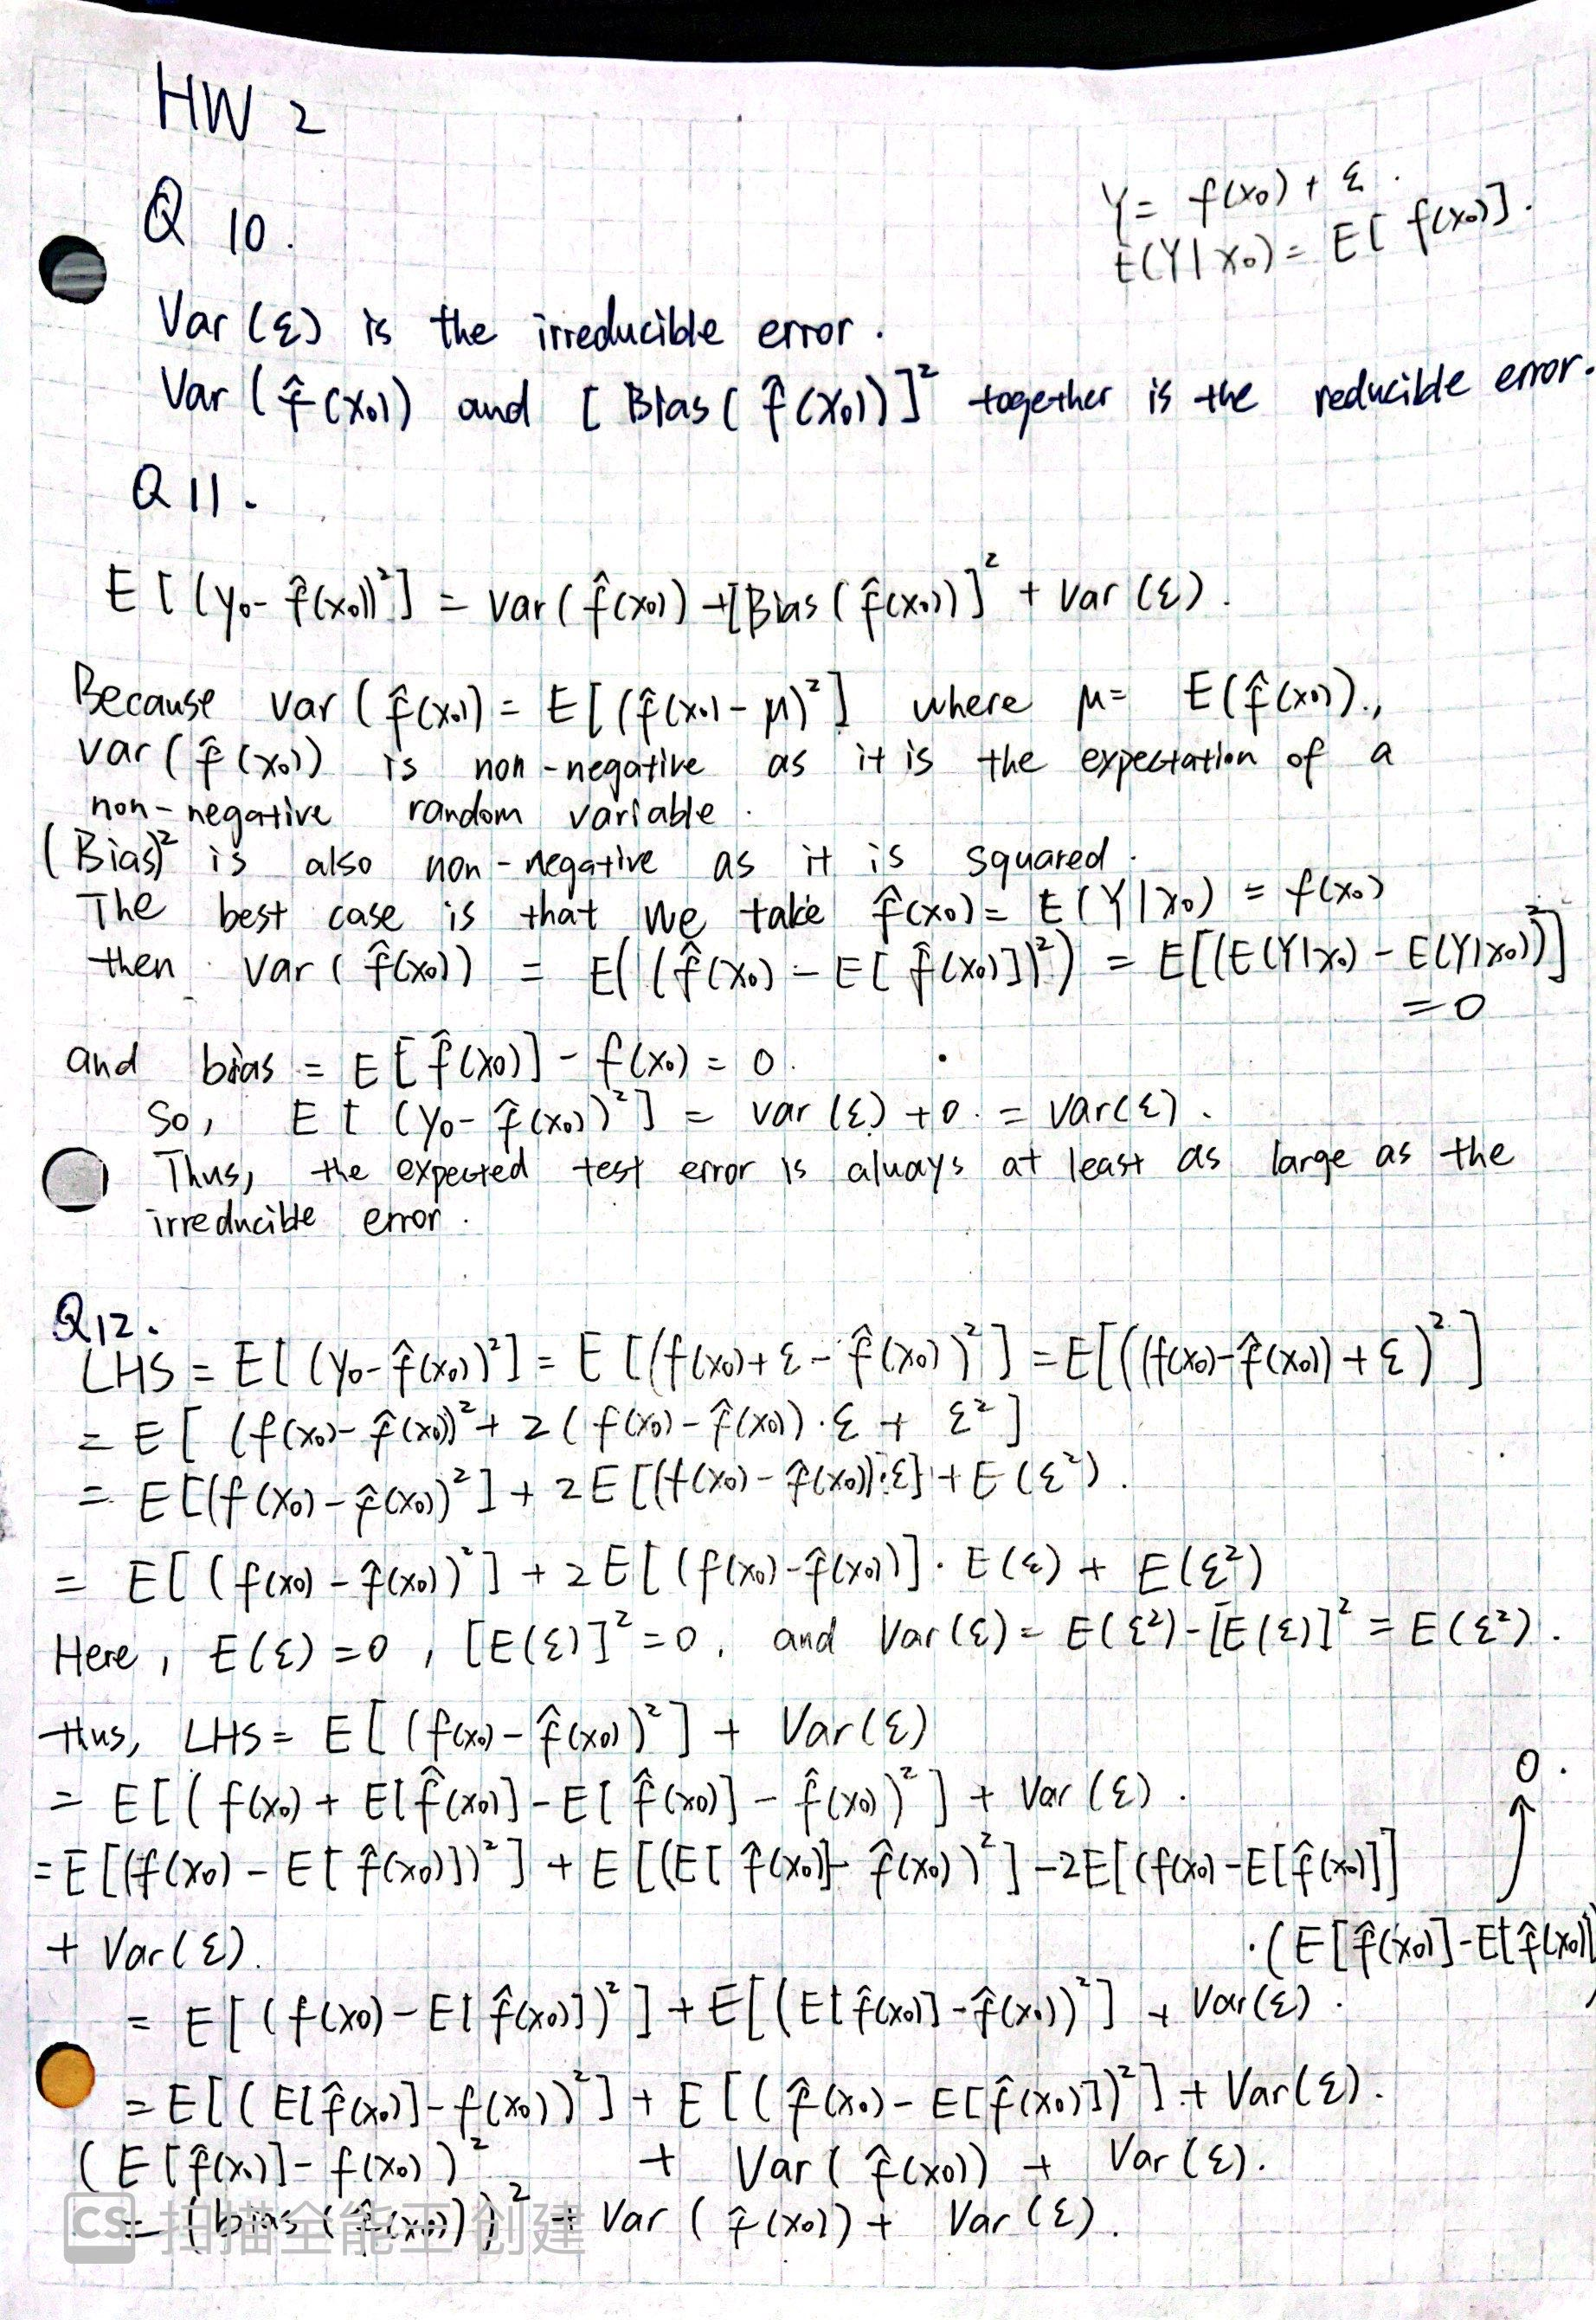
\includegraphics{"C:/Users/26910/Documents/Git/PSTAT-131/week 2/hw2_q10.jpg"}
\caption{Question 10 11 12}
\end{figure}

\end{document}
